\documentclass[12pt]{article}
\usepackage{graphicx}
\usepackage{ragged2e}
\usepackage{array}
\newcolumntype{L}[1]{>{\raggedright\let\newline\\\arraybackslash\hspace{0pt}}m{#1}}
\newcolumntype{C}[1]{>{\centering\let\newline\\\arraybackslash\hspace{0pt}}m{#1}}
\newcolumntype{R}[1]{>{\raggedleft\let\newline\\\arraybackslash\hspace{0pt}}m{#1}}
\begin{document}
	\centering\bf{KOLHAPUR INSTITUTE OF TECHNOLOGY'S}\par
	\bfCOLLEGE OF ENGINEERING (AUTONOMOUS),KOLHAPUR
	\par\noindent\rule{\textwidth}{0.4pt}
	
	\centering\bf{First Year BTech}\par
	\centering\bf{MID SEMESTER EXAMINATION}\par
	\centering\bf{Web Technologies (wt1)}\par
	\begin{flushleft}
		Day and Date :{}\hspace{5.5cm}PRN:
	\end{flushleft}
	
	\begin{flushleft}
		Time :{}\hspace{7cm}Max Marks:{50}\\
	\end{flushleft}
	\noindent\rule{\textwidth}{0.1pt}
\begin{flushleft}
	{\bf Instructions:}\\
	{\hspace{0.5cm} \bf IMP: Verify that you have received question paper with correct course, code, branch, etc}\\
	\hspace{1cm}i) All Questions are Compulsory\\
	\hspace{1cm}ii)Figure to right indicate full marks\\
	\hspace{1cm}iii)Assume suitable data wherever necessary\\
\end{flushleft}

	\begin{flushleft}
	\bf{QNo}\hspace{1.2cm} \bf{Question} \hspace{5.5cm}  \bf{Marks} \hspace{0.2cm} \bf{CO} \hspace{0.2cm}	\bf{BL}	
	
\end{flushleft} 
	\begin{tabular}{|L{1cm}|L{8cm}|C{1cm}|C{1cm}|C{1cm}|}\hline
		\bf{1}. & \bf{Attempt} \bf1 \bf{out} of \bf2 & \bf1  & & \\ \hline
				1.A & What is javascript in default in browser \newline
					
		A)Node.js\newline
		B)Vanilla.js\newline
		C)Script.js\newline
		D)angular.js &
		3 &
		CO1&
		1 \\ \hline
		
				1.B & What are frameworks used for designing web pages? \newline
					
		A)React.js\newline
		B)Node.js\newline
		C)Angular.js\newline
		D)Web.js &
		3 &
		CO5&
		3 \\ \hline
		
		
	\end{tabular}

	\begin{tabular}{|L{1cm}|L{8cm}|C{1cm}|C{1cm}|C{1cm}|}\hline
	\bf2. & \bf{Attempt} \bf{1} \bf{out of} \bf{2} & \bf{1}  & & \\ \hline





		2.A &
	What is meant by a framework? \newline
			
	 &  1 & CO6 & 4\\ \hline
		2.B &
	Where is CSS and where it is used? \newline
			
	 &  2 & CO2 & 3\\ \hline
	\end{tabular}


\begin{tabular}{|L{1cm}|L{8cm}|C{1cm}|C{1cm}|C{1cm}|}\hline
	\bf3. & \bf{Attempt} \bf{1} \bf{out of} \bf{2} & \bf{1}  & & \\ \hline





		3.A &
	image2 question \newline
			\begin{center}
		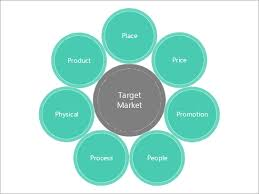
\includegraphics[width=4cm,height=3cm]{media/diagrams/image2.jpg}\\\bf{Figure }\bf3.A		
	\end{center}
		
	 &   & CO4 & 1\\ \hline
		3.B &
	Difference between HTTP and HTTPS. \newline
			
	 &   & CO2 & 3\\ \hline
	\end{tabular}



\end{document}
	
	